% Coloring diagrams - linear relaxation
% Author: Henri Menke
\documentclass[tikz, border=10pt]{standalone}
%%%<
\usepackage{verbatim}
%%%>
\begin{comment}
:Title: Coloring diagrams - linear relaxation
:Tags: Diagrams;Foreach;Shadings;Scopes;
:Author: Henri Menke
:Slug: colored-diagram

TikZ is used for reproducing a diagram by Lê Nguyên Hoang
seen: on http://www.science4all.org/le-nguyen-hoang/integer-programming/ 

The code was written by Henri Menke and published on TeX.SE.
\end{comment}
\usetikzlibrary{shapes}
\begin{document}
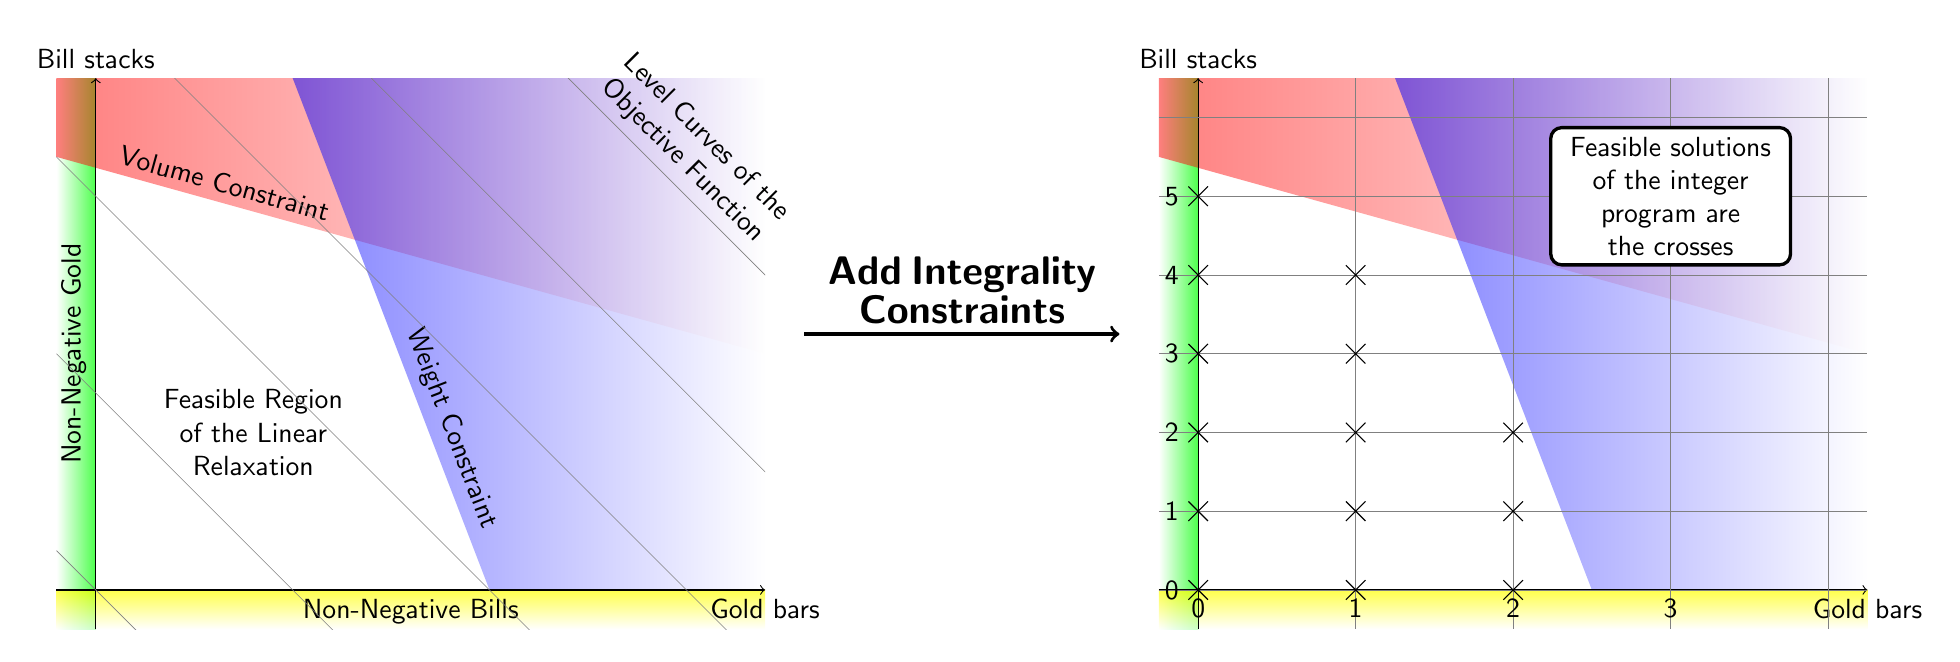
\begin{tikzpicture}[
    every path/.style = {},
    every node/.append style = {font=\sffamily}
  ]
  \begin{scope}
    \shade[right color=green, left color=white, opacity=0.7]
      (-0.5,-0.5) rectangle (0,6.5);
    \node[rotate=90, above] at (0,3) {Non-Negative Gold};
    \shade[top color=yellow, bottom color=white, opacity=0.7]
      (-0.5,-0.5) rectangle (8.5,0);
    \node[below] at (4,0) {Non-Negative Bills};
    \shade[left color=red, bottom color=red, right color=white, opacity=0.5]
      (-0.5,5.5) -- (8.5,3) -- (8.5,6.5) -- (-0.5,6.5) -- cycle;
    \path (-0.5,5.5) -- node[pos=0.23, sloped, above] {Volume Constraint}
      (8.5,3);
    \shade[left color=blue, right color=white, opacity=0.5]
      (2.5,6.5) -- (8.5,6.5) -- (8.5,0) -- (5,0) -- cycle;
    \path (5,0) -- node[pos=0.3, sloped, above] {Weight Constraint} (2.5,6.5);
    \node[text width=7em, align=center] at (2,2)
      {Feasible Region of the Linear Relaxation};
    \draw[->] (-0.5,0) -- (8.5,0) node[below] {Gold bars};
    \draw[->] (0,-0.5) -- (0,6.5) node[above] {Bill stacks};
    \node[rotate=-45, above, text width=9em, align=center] at (7.25,5.25)
      {Level Curves of the Objective Function};
    \path[clip] (-0.5,-0.5) rectangle (8.5,6.5);
    \foreach \i in {0.5,3,...,13} {
      \draw[help lines] (-0.5,\i) -- +(-45:15);
    }
  \end{scope}
  \draw[very thick, ->] (9,3.25) -- node[above, text width=4cm, align=center]
    {\Large\bfseries Add Integrality Constraints} (13,3.25);
  \begin{scope}[shift={(14,0)}]
    \shade[right color=green, left color=white, opacity=0.7]
      (-0.5,-0.5) rectangle (0,6.5);
    \shade[top color=yellow, bottom color=white, opacity=0.7]
      (-0.5,-0.5) rectangle (8.5,0);
    \shade[left color=red, bottom color=red, right color=white, opacity=0.5]
      (-0.5,5.5) -- (8.5,3) -- (8.5,6.5) -- (-0.5,6.5) -- cycle;
   \shade[left color=blue, right color=white, opacity=0.5]
     (2.5,6.5) -- (8.5,6.5) -- (8.5,0) -- (5,0) -- cycle;
    \draw[->] (-0.5,0) -- (8.5,0) node[below] {Gold bars};
    \draw[->] (0,-0.5) -- (0,6.5) node[above] {Bill stacks};
    \foreach \i in {0,1,...,6.5} {
      \draw[help lines] (-0.5,\i) -- (8.5,\i);
    }
    \foreach \i in {2,4,...,8.5} {
      \draw[help lines] (\i,6.5) -- (\i,-0.5);
    }
    \foreach \i in {0,1,...,5} {
      \node[draw,cross out,label={left:\i}] at (0,\i) {};
    }
    \foreach \i in {0,1,...,4} {
      \node[draw,cross out] at (2,\i) {};
    }
    \foreach \i in {0,1,...,2} {
            \node[draw,cross out] at (4,\i) {};
    }
    \foreach \i in {0,2,...,6} {
      \node[below] at (\i,0) {\pgfmathparse{int(\i/2)}\pgfmathresult};
    }
    \node[very thick, draw=black, fill=white, rectangle, rounded corners,
      text width=8em, align=center] at (6,5)
      {Feasible solutions of the integer program are the crosses};
  \end{scope}
\end{tikzpicture}
\end{document}
